\section{Aufbau der Wortuhr}
Nach der mechanischen und elektrischen Vorbereitung, der Konstruktion sowie dem \gls{3ddruck} der Bauteile, erfolgt die Montage des Gesamtsystems.  
Zunächst werden die LED-Streifen zugeschnitten und entsprechend der geplanten Anordnung auf die Grundplatte geklebt.
Hierzu wird das Layout auf die Grundplatte gezeichnet und die positionen der \gls{led}s mit dem zugehörigen Buchstaben bzw. Symbold und den Indizes der \gls{led} beschriftet.
Dadurch kann, ohne die aufgesetzte Frontplatte bei der Inbetriebnahme dauernd abzunehmen und wieder aufzusetzen überprüft werden, ob die korrekten Wörter angezeigt werden und die korrekte \gls{led} angsprochen wird.  
Anschließend werden die einzelnen Streifen durch Lötverbindungen verbunden (vgl. Abb~\ref{fig:VerlötetStreifen}).  
Die Anschluskabel werden auf die Rückseite geführt.  
\begin{figure}[H]
	\centering
	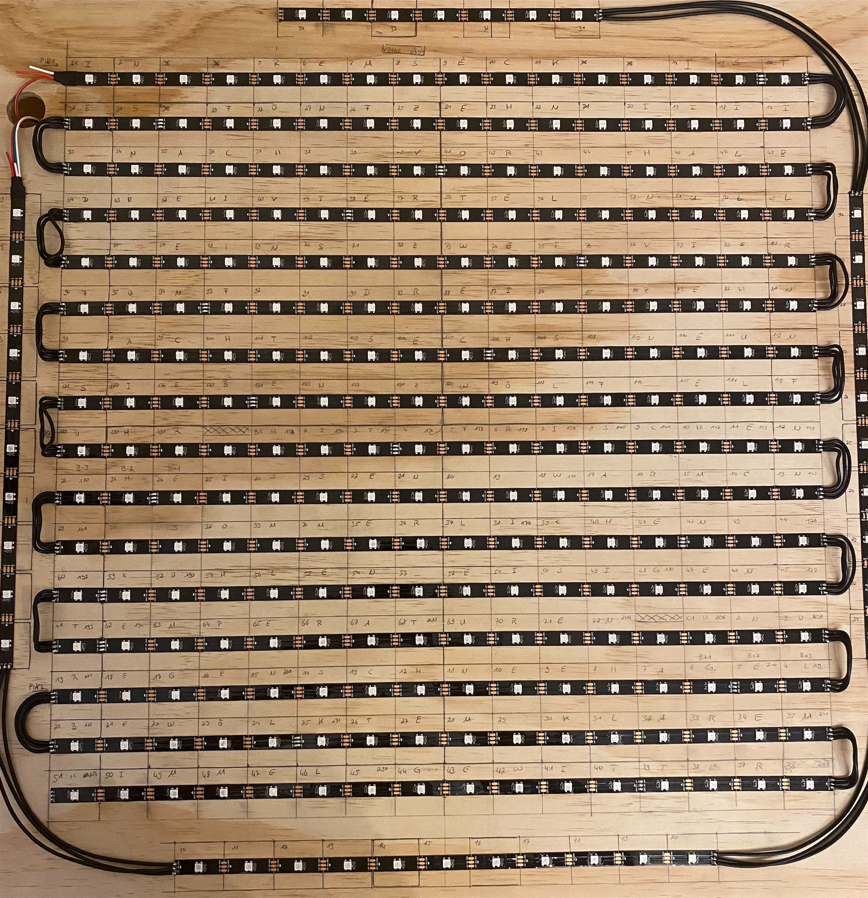
\includegraphics[width=0.7\linewidth]{inhalt/bilder/LEDsVerloetet.png}
	\caption{Alle LED-Streifen auf der Multiplexplatte aufgeklebt und verlötet.}
	\label{fig:VerlötetStreifen}
\end{figure}

Die Verbindung der Frontplatte zur Grundplatte erfolgt über die Eckstteile.  
Hierzu werden Gewindeeinsätze, sogenannte Heatinsert, eingesetzt, welche in das 3D-gedruckte Material integriert werden (vgl. Abb.~\ref{fig:Heatinserts}).
Hierzu werden die Heatinserts z.B. mit einem Lötkolben mit geeigneter Spitze erhitzt und dann eingepresst.
\begin{figure}[H]
	\centering
	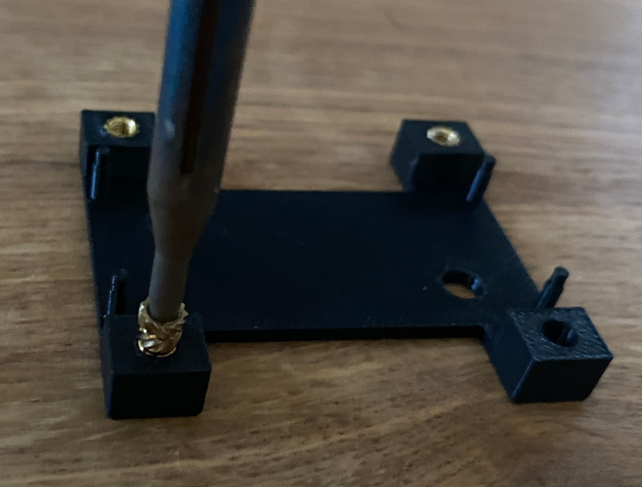
\includegraphics[width=0.7\linewidth]{inhalt/bilder/BeispielHeatinsertESPHalter.png}
	\caption{Einpressvorgang der der Heatinserts am Beispiel des ESP-Halters.}
	\label{fig:Heatinserts}
\end{figure}  
Die Befestigung erfolgt anschließend mit M4x20-Schrauben.  
Die Verbindung der einzelnen Frontplattenbauteile untereinander erfolgt über Durchgangsbohrungen.  
Hierbei werden M3x12-Schrauben in Kombination mit Muttern und Unterlegscheiben verwendet. 

Für die initiale Inbetriebnahme und implementierung der Software wird der Mikrocontroller provisorisch angeschlossen.  
Hierzu werden ein Steckbrett und Jumperkabel verwendet.  
Diese Vorgehensweise ermöglicht eine flexible Anpassung der Verdrahtung während der Testphase.
% Nach erfolgreicher Prüfung aller Funktionen erfolgt die finale Verdrahtung.  
% Die provisorischen Verbindungen werden durch dauerhafte Lötverbindungen ersetzt.